\documentclass[crop,tikz]{standalone}
%\usetikzlibrary{...}% tikz package already loaded by 'tikz' option

\usetikzlibrary{positioning}

 % times is deprecated - using a modern times clone instead
\usepackage{mathptmx}

\begin{document}

% Use monospace font (Latin Modern Typewriter) for all text.
% Source: https://tex.stackexchange.com/a/25251
%{\fontfamily{lmtt}\selectfont

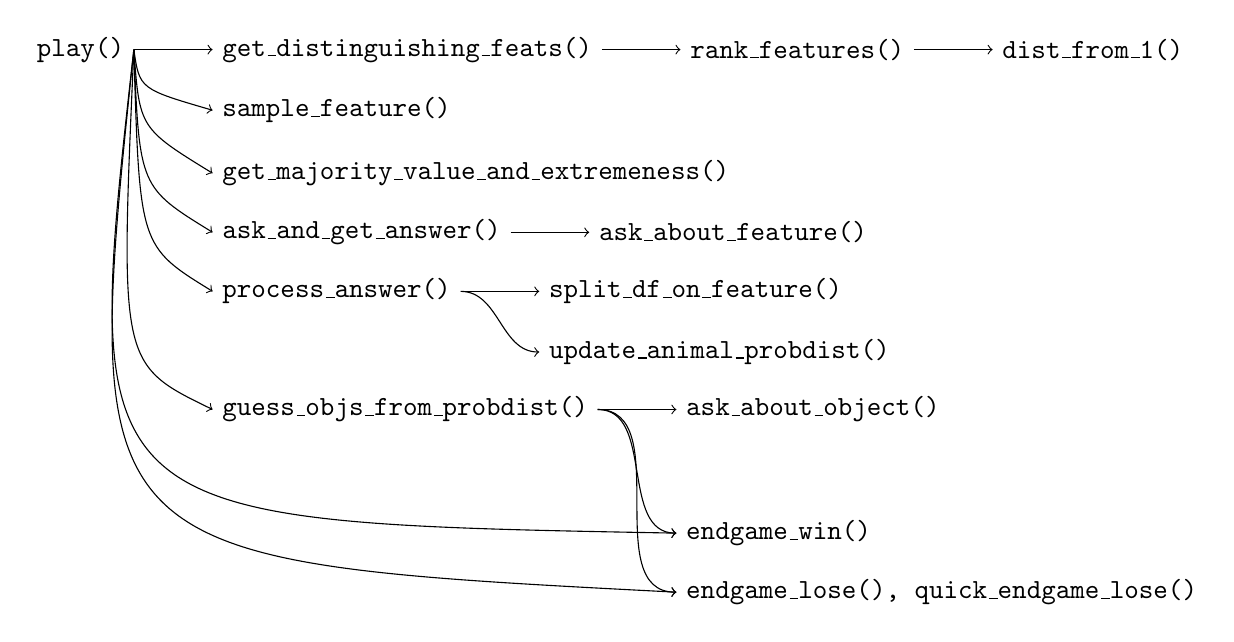
\begin{tikzpicture}

% ======================================
% THE PLAY NODE
% ======================================
\node (play) at (0,0) {\texttt{play()}};

% ======================================
% BLOCK 1 (TEAL): SAMPLING FEATURES
% ======================================

\node[right=1cm of play] (gdf) {\texttt{get\_distinguishing\_feats()}};
\node[right=1cm of gdf] (rf) {\texttt{rank\_features()}};
\node[right=1cm of rf] (df1) {\texttt{dist\_from\_1()}};
\draw [->] (play.east) -- (gdf.west);
\draw [->] (gdf.east) -- (rf.west);
\draw [->] (rf.east) -- (df1.west);

\node[below right=0.2cm and 1cm of play] (sf) {\texttt{sample\_feature()}};
\draw [->] (play.east) .. controls (0.75, -0.5) .. (sf.west);

% ======================================
% BLOCK 2 (GREEN): ASK ABOUT FEATURE AND PROCESS ANSWER
% ======================================

\node[below right=1cm and 1cm of play] (gmvae) {\texttt{get\_majority\_value\_and\_extremeness()}};
\draw [->] (play.east) .. controls (0.75, -1) .. (gmvae.west);

\node[below right=1.75cm and 1cm of play] (aaga) {\texttt{ask\_and\_get\_answer()}};
\node[right=1cm of aaga] (aaf) {\texttt{ask\_about\_feature()}};
\draw [->] (play.east) .. controls (0.75, -1.75) .. (aaga.west);
\draw [->] (aaga.east) -- (aaf.west);

\node[below right=2.5cm and 1cm of play] (pa) {\texttt{process\_answer()}};
\node[right=1cm of pa] (sdof) {\texttt{split\_df\_on\_feature()}};
\node[below right=0.2cm and 1 cm of pa] (uap) {\texttt{update\_animal\_probdist()}};
\draw [->] (play.east) .. controls (0.75, -2.5) .. (pa.west);
\draw [->] (pa.east) -- (sdof.west);
\draw [->] (pa) to [out=0, in=180] (uap);

% ======================================
% BLOCK 3 (LILAC): ASK ABOUT ANIMALS
% ======================================
	
\node[below right=4cm and 1cm of play] (gofp) {\texttt{guess\_objs\_from\_probdist()}};
\node[right=1cm of gofp] (aao) {\texttt{ask\_about\_object()}};
\draw [->] (play.east) .. controls (0.5, -4) .. (gofp.west);
\draw [->] (gofp.east) -- (aao.west);

% ======================================
% BLOCK 3 (SALMON): ENDGAME
% ======================================

\node[below right=1cm and 1cm of gofp] (ew) {\texttt{endgame\_win()}};
\node[below right=1.75cm and 1cm of gofp] (el) {\texttt{endgame\_lose(), quick\_endgame\_lose()}};
\draw [->] (play.east) .. controls (0, -6) .. (ew.west);
\draw [->] (play.east) .. controls (0, -6.5) .. (el.west);
\draw [->] (gofp) to [out=0, in=180] (ew);
\draw [->] (gofp) to [out=0, in=180] (el);

\end{tikzpicture}

%}
	
\end{document}